\documentclass{beamer}

%
% Escolha o formato da  sua Apresenta��o 
%
% Para mais temas, esquemas de cores e fontes, veja:
% http://deic.uab.es/~iblanes/beamer_gallery/index_by_theme.html
% (link em Ingl�s)
%

\mode<presentation>
{
  \usetheme{Warsaw}       
  % escolha do tema, experimente Darmstadt, Madrid, Dresden, ...
  \usecolortheme{default} 
  % escolha do esquema de cor, experimente albatross, beaver, crane, ...
  \usefonttheme{default}  
  % escolha da fontes, experimente serif, structurebold, ...
  \setbeamertemplate{navigation symbols}{}
  \setbeamertemplate{caption}[numbered]
} 

\usepackage[brazil]{babel}
\usepackage[utf8x]{inputenc}

\title{Revolu��o dos Cravos}
\author{Otelo Saraiva de Carvalho}
\institute{Portugal}
\date{25 de Abril 1975}

\begin{document}

\begin{frame}
  \titlepage
\end{frame}



\begin{frame}{Ind�ce}
  \tableofcontents
\end{frame}

\section{Agenda}

\begin{frame}{Agenda}

\begin{itemize}
  \item Prepara��o do Golpe 
  \item Movimenta��es Militares
  \item Restaurar o Governo
\end{itemize}

\end{frame}

\begin{frame}{Fora da Agenda!}

\begin{itemize}[<+->]
  \item Assalto ao Castelo
  \item Viol�ncia nas Ruas
  \item Dispers�o de Manifestantes
\end{itemize}

\end{frame}

\section{Revis�o}

\begin{frame}{Objectivos principais \& Fatores de Sucesso}

\begin{itemize}
\item O que faz uma na��o �nica:
  \begin{itemize}
    \item Liberdade
    \item Todos os Homens s�o iguais
  \end{itemize}
\end{itemize}

\begin{block}{Vis�o comum}
\begin{itemize}
\item Restauro da Liberdade.
\item Um governo para/pelo o povo.
\end{itemize}
\end{block}

\end{frame}

\begin{frame}{Resultados}

\begin{figure}
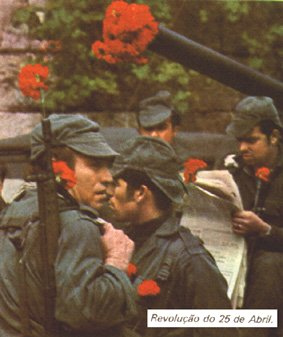
\includegraphics[width=0.3\textwidth]{Cravos.jpg}
\end{figure}

\begin{block}{N�mero de Mortes}
\begin{equation}
(4 \times 20 - 73) = 7
\end{equation}
\end{block}

\end{frame}

\section{Sum�rio}

\begin{frame}{Sum�rio}

\begin{columns}
\begin{column}{0.6\textwidth}
\begin{itemize}
\item Revolu��o Pac�fica
\item Implanta��o da Rep�blica
\item Fim da Guerra Colonial
\end{itemize}
\end{column}
\begin{column}{0.4\textwidth}
\begin{itemize}
\item Liberdade
\item Uni�o
\item Fraternidade
\end{itemize}
\end{column}
\end{columns}

\end{frame}

\end{document}